\apendice{Plan de Proyecto Software}
\label{apendice:plan-proyecto-software}

\section{Introducción}
\label{sec:a-introduccion}

Este apartado describe la planificación, organización, viabilidad y gestión de riesgos seguidas durante el desarrollo del proyecto. El objetivo de este anexo es documentar no solo la planificación inicial, sino también la evolución real del trabajo a lo largo de las distintas iteraciones, considerando las desviaciones, ajustes técnicos y decisiones de refactorización que se produjeron durante el desarrollo.

El sistema desarrollado se ha estructurado como una suite de software formada por dos complementos o \textit{add-ons} independientes y complementarios para el entorno de modelado 3D Blender~\cite{blenderapi}:

\begin{itemize}
    \item \textbf{Data Logger 3D o módulo de recopilación:} encargado de registrar automáticamente y en segundo plano la actividad técnica del usuario durante sesiones de modelado 3D. Este add-on captura eventos, estados, transformaciones espaciales, cambios topológicos, operaciones relevantes, cambios de modo, modificaciones UV y otros indicadores asociados al proceso de modelado. Los datos se almacenan en formato CSV para su posterior análisis.

    \item \textbf{Add-on de análisis y visualización:} encargado de procesar de forma diferida los CSV generados por el logger. Este segundo componente lee y valida los datos, calcula métricas estadísticas A1--A17, métricas geométricas, métricas UV y genera resultados visuales mediante paneles, gráficos y visualizaciones integradas en Blender.
\end{itemize}

Esta división modular permite separar la fase de adquisición de datos de la fase de interpretación. La captura debe ser ligera, estable y poco intrusiva, ya que se ejecuta durante la sesión de modelado. En cambio, el análisis puede incorporar operaciones más costosas, como cálculos estadísticos, comparaciones geométricas, generación de gráficos y visualizaciones 3D, porque se ejecuta posteriormente y bajo demanda.

El proyecto se ha llevado a cabo mediante un \textbf{enfoque iterativo e incremental}, construyendo inicialmente versiones de funcionalidad mínima viable que posteriormente han sido refinadas y ampliadas. Esta estrategia permitió detectar problemas de forma temprana, especialmente en relación con la API de Blender, la gestión de modos de edición, la captura de eventos y la validación de métricas. Asimismo, facilitó que el alcance evolucionara desde un registrador básico de actividad hacia una suite completa de captura, análisis y visualización.

Para la gestión del código se ha utilizado GitHub~\cite{github}, lo que ha permitido mantener un historial de commits con la evolución del proyecto. Este historial se ha empleado como fuente de contraste para revisar la planificación y comprobar qué tareas fueron ejecutadas realmente en cada etapa. La documentación se ha redactado y maquetado en \LaTeX~\cite{wiki:latex}, siguiendo la estructura institucional del Trabajo de Fin de Grado.

\section{Planificación temporal}
\label{sec:a-planificacion-temporal}

El desarrollo se organizó en ciclos de trabajo o \textit{sprints}, con una orientación aproximada quincenal. Cada iteración incorporó nuevas funcionalidades o mejoras sobre la base existente. La planificación inicial partía de una evolución progresiva: primero un logger funcional, después la normalización del CSV, posteriormente el análisis de datos y finalmente la visualización, validación y refinamiento de interfaz.

No obstante, la ejecución real mostró que varias tareas tuvieron que redistribuirse entre sprints. La razón principal fue la complejidad técnica del entorno Blender, especialmente en la detección de eventos internos, el comportamiento diferente entre \textit{Object Mode} y \textit{Edit Mode}, la captura de UV y el cálculo correcto de métricas a partir de CSV reales. Por ello, la planificación se mantuvo como una guía de trabajo, pero la ejecución siguió un patrón incremental y adaptativo.

\subsection{Fase previa}
\label{subsec:a-fase-previa}

Durante la fase previa se realizó el estudio inicial de viabilidad técnica y el análisis del entorno de ejecución de Blender. Se revisaron las posibilidades ofrecidas por la API \texttt{bpy}, los operadores internos de Blender, los manejadores persistentes y los mecanismos de acceso a objetos, mallas, modos de edición y transformaciones.

El objetivo previsto era comprobar si resultaba viable registrar actividad técnica de una sesión de modelado sin interferir en el flujo de trabajo del usuario. Esta fase permitió confirmar que la solución era viable, aunque también se detectó una limitación importante: Blender no proporciona todos los eventos de modelado de forma directa y homogénea. Esta dificultad condicionó decisiones posteriores, como la comparación de estados mediante \textit{snapshots}, el uso de temporizadores, la detección de operadores recientes y el empleo de \texttt{bmesh} para acceder correctamente a mallas en modo edición.

\subsection{Sprint 0: definición inicial del proyecto}
\label{subsec:a-sprint-0}

El Sprint 0 se dedicó a la definición del dominio del problema, el alcance funcional y la arquitectura inicial. En esta etapa se planteó la separación del sistema en dos add-ons independientes:

\begin{itemize}
    \item un primer add-on centrado en la recopilación de datos durante el modelado;
    \item un segundo add-on orientado al análisis posterior de los registros generados.
\end{itemize}

La planificación prevista consistía en delimitar requisitos, establecer el formato de intercambio y definir el flujo general de datos. La ejecución real confirmó la validez de esta separación, aunque el desarrollo posterior mostró que el segundo add-on tendría un peso mayor del inicialmente previsto. El módulo de análisis no se limitó a leer CSV, sino que terminó incorporando validación de datos, métricas estadísticas, métricas geométricas, métricas UV, gráficos, visualizaciones y una interfaz organizada por pestañas.

\subsection{Sprint 1: primera versión funcional del Data Logger 3D}
\label{subsec:a-sprint-1}

El primer sprint de desarrollo se centró en crear una primera versión funcional del add-on de captura. El objetivo previsto era disponer de un prototipo mínimo capaz de ejecutarse dentro de Blender, mostrar una interfaz básica y registrar datos en formato CSV.

Las tareas previstas fueron:

\begin{itemize}
    \item creación de la estructura inicial del add-on;
    \item definición de operadores básicos;
    \item incorporación de una interfaz gráfica inicial;
    \item captura de eventos o estados relevantes;
    \item escritura inicial de registros en CSV.
\end{itemize}

La ejecución real se ajustó de forma razonable a lo planificado. El historial de commits refleja una primera versión de \textit{Data Logger 3D} y una interfaz gráfica básica durante el mes de febrero. Esta etapa permitió obtener un prototipo inicial funcional, aunque todavía limitado en cuanto a precisión, robustez y normalización de datos.

El resultado principal fue una primera base operativa sobre la que se pudieron construir las versiones posteriores. Sin embargo, la experiencia adquirida en este sprint también evidenció que la captura de datos en Blender requería una aproximación más cuidadosa que una simple lectura periódica de valores. Era necesario distinguir cambios reales de estados repetidos, evitar registros redundantes y controlar el impacto en el rendimiento.

\subsection{Sprint 2: refinamiento de captura y normalización del CSV}
\label{subsec:a-sprint-2}

El segundo sprint se planificó como una fase de refinamiento del logger. El objetivo principal era mejorar la captura de eventos, reorganizar los datos registrados y avanzar hacia una estructura CSV más estable.

Las tareas previstas fueron:

\begin{itemize}
    \item corregir errores de versiones iniciales;
    \item mejorar el registro de eventos significativos;
    \item reorganizar archivos del proyecto;
    \item avanzar en la normalización del CSV;
    \item preparar el formato de datos para el futuro add-on de análisis.
\end{itemize}

La ejecución real se centró especialmente en corregir versiones tempranas y reorganizar el código. En esta fase se realizaron movimientos de archivos, eliminación de componentes obsoletos y ajustes relacionados con la captura de eventos significativos. Esta desviación respecto a una planificación puramente funcional resultó positiva, ya que permitió reducir ruido en los datos y preparar una base más coherente para las métricas posteriores.

El principal aprendizaje de este sprint fue que el CSV debía tratarse como un contrato entre los dos add-ons. Cualquier cambio en la estructura del logger afectaría directamente al análisis posterior, por lo que la cabecera, los campos registrados y la semántica de cada columna debían mantenerse documentados y controlados.

\subsection{Sprint 3: implementación inicial del add-on de análisis}
\label{subsec:a-sprint-3}

El tercer sprint tuvo como objetivo iniciar el segundo add-on de la suite. La planificación contemplaba la lectura de CSV, el cálculo de primeras métricas temporales y espaciales, y una interfaz inicial para el análisis.

Las tareas previstas fueron:

\begin{itemize}
    \item crear la estructura base del add-on de análisis;
    \item implementar la lectura de archivos CSV;
    \item calcular primeras métricas temporales y espaciales;
    \item mostrar resultados básicos en Blender;
    \item preparar primeras visualizaciones.
\end{itemize}

La ejecución real incorporó varias versiones asociadas a la implementación del análisis temporal y espacial. También se subieron archivos ZIP del add-on de análisis, se eliminaron versiones antiguas y se reorganizaron carpetas. Esto indica que el sprint no solo permitió implementar cálculo analítico, sino también consolidar la estructura del segundo complemento.

Durante esta fase comenzaron a aparecer problemas propios del análisis de datos: valores incompletos, necesidad de interpretar columnas temporales, cálculo de velocidades, distancias y evolución de actividad. Por ello, la implementación inicial tuvo que combinar lectura de datos, depuración de CSV y primeras decisiones sobre cómo presentar los resultados.

\subsection{Sprint 4: métricas, visualización inicial y evolución del logger}
\label{subsec:a-sprint-4}

El cuarto sprint se planificó como una fase de ampliación de métricas y primeras visualizaciones. El objetivo previsto era avanzar en el cálculo de métricas temporales, espaciales y topológicas, además de desarrollar elementos gráficos iniciales.

Las tareas previstas fueron:

\begin{itemize}
    \item ampliar métricas temporales y espaciales;
    \item iniciar métricas topológicas;
    \item mejorar gráficos y ejes 3D;
    \item probar el análisis con datos de prueba;
    \item continuar la documentación técnica.
\end{itemize}

La ejecución real combinó estas tareas con una evolución importante del logger. Se incorporaron mejoras en ejes 3D, datos de prueba reales y actualizaciones de documentación. Además, el logger avanzó hacia una versión más robusta, incorporando cambios significativos en la detección de eventos, el sistema de logging y la interfaz de control.

Este sprint muestra una primera desviación clara: parte del esfuerzo previsto para análisis y visualización tuvo que compartirse con la mejora del sistema de captura. La causa fue técnica: si el logger no registraba correctamente los eventos, las métricas calculadas posteriormente podían perder precisión o resultar inconsistentes. Por tanto, se priorizó reforzar la calidad de los datos de entrada antes de ampliar excesivamente la capa de análisis.

\subsection{Sprint 5: refactorización del logger y soporte avanzado de Blender}
\label{subsec:a-sprint-5}

El quinto sprint se centró en la refactorización profunda del subsistema de captura. El objetivo era mejorar la robustez del logger, especialmente en relación con \textit{Edit Mode}, operadores de Blender, deltas, UV y persistencia CSV.

Las tareas previstas fueron:

\begin{itemize}
    \item incorporar soporte para \textit{Edit Mode} mediante \texttt{bmesh};
    \item mejorar la detección de operadores como \texttt{Ctrl+V}, \texttt{Shift+D}, \texttt{Alt+D} y \texttt{Merge};
    \item detectar cambios UV;
    \item reducir registros redundantes;
    \item añadir controles de inicio y parada;
    \item incorporar un panel de depuración;
    \item corregir el registro de deltas en \textit{Object Mode}.
\end{itemize}

La ejecución real confirma que este sprint fue uno de los más relevantes desde el punto de vista técnico. Se corrigió el registro de deltas en \textit{Object Mode}, evitando perder cambios al borrar objetos. También se restauró el comportamiento nativo de \textit{Shift+D} y \textit{Alt+D}, se mejoró el sistema de logging, se añadió detección robusta de UV y se incorporó un panel de depuración.

La revisión de este sprint muestra que el objetivo se cumplió, aunque con mayor complejidad de la prevista. La diferencia entre los modos de Blender obligó a utilizar estrategias distintas para leer la malla en modo objeto y en modo edición. Además, algunas operaciones de usuario no podían capturarse únicamente mediante cambios de contadores, por lo que fue necesario combinar detección de operadores, banderas internas, hash UV y comparación de \textit{snapshots}.

El resultado fue una versión mucho más estable del logger, capaz de registrar únicamente cambios significativos y reducir el crecimiento innecesario del CSV.

\subsection{Sprint 6: análisis avanzado, métricas y gráficos}
\label{subsec:a-sprint-6}

El sexto sprint se dedicó al desarrollo avanzado del add-on de análisis. La planificación contemplaba la ampliación del cálculo estadístico, la incorporación de métricas sobre CSV y la generación de gráficos enriquecidos.

Las tareas previstas fueron:

\begin{itemize}
    \item implementar análisis estadístico de CSV;
    \item calcular media, mediana, desviación estándar, mínimos y máximos cuando procediera;
    \item ampliar métricas A1--A17;
    \item incorporar visualizaciones con Matplotlib~\cite{matplotlib};
    \item mejorar la presentación de resultados en la interfaz;
    \item actualizar la documentación técnica.
\end{itemize}

La ejecución real incluyó la incorporación de análisis estadístico de CSV, actualización de métricas y mejoras de documentación. Se añadieron cálculos descriptivos y se avanzó en la representación gráfica. No obstante, algunas funciones de cálculo de métricas CSV necesitaron correcciones posteriores, especialmente cuando se aplicaron a múltiples CSV o a datos reales.

La revisión de este sprint evidencia que el cálculo de métricas no fue una tarea cerrada en una única iteración. Fue necesario ajustar funciones, validar entradas, controlar valores no numéricos y revisar la interpretación de los resultados. Esta situación es coherente con la naturaleza incremental del proyecto: la validez de las métricas dependía tanto del formato del CSV como de la variedad de sesiones analizadas.

\subsection{Sprint 7: validación con datos reales y corrección de métricas}
\label{subsec:a-sprint-7}

El séptimo sprint se planificó como una fase de validación, pruebas funcionales y corrección de defectos. El objetivo era comprobar el comportamiento del sistema con datos reales y mejorar la estabilidad de las métricas.

Las tareas previstas fueron:

\begin{itemize}
    \item validar el sistema con CSV reales;
    \item comprobar el cálculo de métricas A1--A17;
    \item revisar el análisis de múltiples CSV;
    \item corregir errores de cálculo;
    \item integrar el segundo add-on en la documentación;
    \item preparar el sistema para su cierre.
\end{itemize}

La ejecución real muestra la incorporación de datos reales de actividad con la EASD de Burgos, así como varias correcciones sobre \texttt{Calculate CSV Metric Stats} y métricas CSV múltiples. También se llevó a cabo la reestructuración de anexos e integración completa del segundo add-on en la documentación del TFG.

Este sprint cumplió su función de validación, pero también reveló errores que no habían aparecido en pruebas más controladas. La lectura de CSV múltiples y el cálculo estadístico sobre datos reales exigieron revisar funciones, controlar casos límite y reforzar la validación. Por tanto, la ejecución real fue más correctiva de lo previsto, pero permitió aumentar la fiabilidad del sistema antes de la fase final.

\subsection{Sprint 8: cierre, refactorización final e interfaz por pestañas}
\label{subsec:a-sprint-8}

El último sprint se dedicó a la consolidación de la suite completa. La planificación contemplaba el refinamiento de la interfaz, la revisión de documentación, la corrección de errores pendientes y la preparación de la versión final.

Las tareas previstas fueron:

\begin{itemize}
    \item revisar la documentación final;
    \item mejorar la interfaz del add-on de análisis;
    \item eliminar redundancias visuales;
    \item incorporar textos breves y tooltips;
    \item organizar resultados de forma más clara;
    \item cerrar una versión estable de la suite.
\end{itemize}

La ejecución real incluyó una refactorización final importante. Se reorganizó la estructura interna del código, separando la lógica de cálculo, la interfaz y la generación de visualizaciones. También se incorporaron optimizaciones mediante estructuras tipo KDTree para mejorar cálculos geométricos relacionados con búsquedas de proximidad entre mallas. Además, se revisaron funciones de métricas procedentes de CSV y métricas de malla, incluyendo similitud, distancia de Hausdorff, normales, ángulos, duplicados de vértices y métricas UV.

En la interfaz se incorporó una organización por pestañas, separando la navegación entre métricas estadísticas, métricas geométricas, métricas UV y visualizaciones. Esta decisión mejoró la claridad del add-on y redujo la sobrecarga visual. El sprint cumplió su objetivo de cierre, aunque también asumió tareas de optimización técnica que inicialmente podrían haberse previsto en fases anteriores.

El resultado final fue una suite más organizada, mantenible y coherente, con una separación más clara entre captura, análisis, cálculo geométrico e interfaz.

\subsection{Resumen de sprints}
\label{subsec:a-resumen-sprints}

La Tabla~\ref{tab:sprints_resumen} sintetiza de forma cronológica las fases fundamentales que han articulado el ciclo de vida del desarrollo.

\begin{table}[H]
\centering
\scriptsize
\renewcommand{\arraystretch}{1.25}
\begin{tabularx}{\textwidth}{p{2cm}p{2.4cm}X X}
\toprule
\textbf{Sprint} & \textbf{Periodo} & \textbf{Funcionalidades principales} & \textbf{Resultado} \\
\midrule
Fase previa & Noviembre & Estudio de Blender, API \texttt{bpy}, eventos y viabilidad técnica. & Confirmación de viabilidad y detección de limitaciones iniciales. \\
Sprint 0 & Enero & Requisitos, alcance y arquitectura basada en dos add-ons. & Definición del enfoque modular. \\
Sprint 1 & Febrero 1--2 & Logger inicial, interfaz básica y CSV. & Primera versión funcional del sistema de captura. \\
Sprint 2 & Febrero 3--4 & Refinamiento de captura, reorganización y normalización CSV. & Base más estable para el intercambio de datos. \\
Sprint 3 & Marzo 1--2 & Add-on de análisis, lectura CSV y primeras métricas. & Integración inicial del análisis temporal y espacial. \\
Sprint 4 & Marzo 3--4 & Métricas, ejes 3D, pruebas y evolución del logger. & Mejora simultánea de análisis y captura. \\
Sprint 5 & Abril 1--2 & Refactorización del logger, \texttt{bmesh}, operadores, UV y deltas. & Versión avanzada y robusta del Data Logger 3D. \\
Sprint 6 & Abril 3--4 & Análisis estadístico, métricas CSV y gráficos. & Add-on de análisis más completo. \\
Sprint 7 & Mayo 1--2 & Validación con datos reales y corrección de métricas. & Sistema validado y funciones corregidas. \\
Sprint 8 & Mayo 3--4 & Refactorización final, KDTree, pestañas, documentación e interfaz. & Versión final de la suite completa. \\
\bottomrule
\end{tabularx}
\caption{Resumen cronológico de los sprints del proyecto.}
\label{tab:sprints_resumen}
\end{table}

\subsection{Revisión de ejecución por sprint}
\label{subsec:a-revision-sprints}

La revisión de cada sprint se ha realizado contrastando la planificación prevista con la evolución real reflejada en el historial de commits. Este análisis permite observar que el desarrollo mantuvo una orientación incremental, aunque algunas tareas se desplazaron entre iteraciones debido a la complejidad técnica de Blender, la depuración de métricas y la necesidad de reorganizar progresivamente la arquitectura del sistema.

\begin{table}[H]
\centering
\scriptsize
\renewcommand{\arraystretch}{1.25}
\begin{tabularx}{\textwidth}{p{2cm}p{4.2cm}X}
\toprule
\textbf{Sprint} & \textbf{Plan previsto} & \textbf{Ejecución real y revisión} \\
\midrule

\textbf{Fase previa} &
Analizar la viabilidad técnica del proyecto y comprobar si era posible registrar eventos y transformaciones en Blender. &
La fase permitió confirmar la viabilidad general, pero también mostró que la API de Blender no ofrece todos los eventos de forma directa. Esta limitación justificó el uso posterior de temporizadores, comparación de estados, operadores internos y estructuras \texttt{bmesh}. \\

\midrule

\textbf{Sprint 0} &
Definir requisitos, alcance y arquitectura inicial basada en dos add-ons. &
La separación entre logger y análisis se mantuvo durante todo el proyecto. Sin embargo, el segundo add-on adquirió más alcance del previsto al incorporar validación, métricas geométricas, métricas UV, gráficos e interfaz por pestañas. \\

\midrule

\textbf{Sprint 1} &
Crear una primera versión funcional del logger con interfaz básica y salida CSV. &
Se consiguió una primera versión operativa de Data Logger 3D. La ejecución fue coherente con el plan, aunque el prototipo inicial requería mejoras importantes en precisión, persistencia y reducción de registros redundantes. \\

\midrule

\textbf{Sprint 2} &
Mejorar la captura, reorganizar el proyecto y normalizar el CSV. &
El trabajo real se orientó a corregir versiones tempranas, mover archivos, eliminar elementos obsoletos y registrar únicamente eventos significativos. Esta reorganización fue necesaria para estabilizar la base del proyecto. \\

\midrule

\textbf{Sprint 3} &
Implementar el add-on de análisis, leer CSV y calcular primeras métricas. &
Se implementó el análisis temporal y espacial, se mejoró la interfaz y se consolidó la estructura del segundo add-on. También se subieron paquetes ZIP y se eliminaron versiones antiguas, lo que reflejó una fase de reorganización además de implementación. \\

\midrule

\textbf{Sprint 4} &
Ampliar métricas y desarrollar primeras visualizaciones. &
Además de trabajar en ejes 3D, datos de prueba y documentación, se reforzó el logger. Parte del esfuerzo previsto para análisis se dedicó a mejorar la captura, ya que la calidad del CSV condicionaba la validez de las métricas posteriores. \\

\midrule

\textbf{Sprint 5} &
Refactorizar el logger, mejorar \textit{Edit Mode}, operadores, UV y deltas. &
La ejecución confirmó la complejidad del logger. Se corrigieron deltas en \textit{Object Mode}, se restauró el comportamiento nativo de duplicaciones, se mejoró la detección de operadores y se añadió soporte robusto para UV y depuración. \\

\midrule

\textbf{Sprint 6} &
Desarrollar análisis estadístico, métricas CSV y visualizaciones. &
Se incorporaron estadísticas descriptivas y métricas sobre CSV. No obstante, algunas funciones requirieron correcciones posteriores al probarse con varios CSV y datos más diversos. \\

\midrule

\textbf{Sprint 7} &
Validar con datos reales, corregir errores y estabilizar el sistema. &
Se añadieron datos reales de actividad y se corrigieron funciones de cálculo de métricas CSV múltiples. La validación mostró errores no detectados en pruebas iniciales y obligó a reforzar la lógica analítica. \\

\midrule

\textbf{Sprint 8} &
Cerrar documentación, refinar interfaz y preparar versión final. &
Además del cierre documental, se realizó una refactorización profunda. Se separó cálculo, interfaz y visualización, se incorporaron optimizaciones con KDTree, se corrigieron métricas CSV y de mallas, y se reorganizó la interfaz mediante pestañas. \\

\bottomrule
\end{tabularx}
\caption{Revisión de ejecución por sprint a partir de la planificación.}
\label{tab:revision-sprints}
\end{table}

En conjunto, la revisión muestra que la planificación inicial se mantuvo como guía general, pero el desarrollo real evolucionó de forma más iterativa de lo previsto. Las principales desviaciones no se debieron a cambios arbitrarios de alcance, sino a problemas técnicos detectados durante la integración con Blender, especialmente en la captura de eventos, la gestión de modos de edición, la validación de CSV y el cálculo de métricas geométricas. Esta evolución permitió mejorar la robustez del sistema y llegar a una versión final más completa que la inicialmente planteada.

\subsection{Tabla de desviaciones: planificación frente a ejecución}
\label{subsec:a-desviaciones}

La Tabla~\ref{tab:desviaciones} expone las desviaciones temporales más relevantes detectadas durante el ciclo de vida del software, contrastando hitos planificados con resultados reales.

\begin{table}[H]
\centering
\scriptsize
\renewcommand{\arraystretch}{1.2}
\begin{tabularx}{\textwidth}{p{3.3cm}p{1.8cm}p{1.8cm}p{1.6cm}X}
\toprule
\textbf{Hito técnico} & \textbf{Plan.} & \textbf{Real} & \textbf{Desv.} & \textbf{Justificación técnica} \\
\midrule
Prototipo inicial del logger & 16 Feb & 16 Feb & 0 d & Se alcanzó una primera versión funcional con interfaz básica y registro inicial. \\
Implementación v0.3 & 05 Mar & 11 Mar & +6 d & La lectura de CSV, el análisis temporal y espacial y la reorganización del add-on de análisis requirieron más iteraciones de las previstas. \\
Soporte avanzado de \textit{Edit Mode} & 10 Mar & 20 Mar & +10 d & La lectura de mallas editables mediante \texttt{bmesh} y la detección robusta de eventos resultaron más complejas de lo esperado. \\
Análisis estadístico CSV & 20 Abr & 27 Abr & +7 d & La integración de estadísticas descriptivas y validación de datos exigió revisar funciones de cálculo. \\
Validación con datos reales & 10 May & 15 May & +5 d & Los CSV reales revelaron errores en métricas múltiples y obligaron a corregir funciones de cálculo. \\
Documentación e interfaz final & 15 May & 18 May & +3 d & El refinamiento de la interfaz, la mejora de gráficos comparativos y la actualización documental se extendieron hasta la fase final. \\
Refactorización final y KDTree & 20 May & 26 May & +6 d & La reorganización entre cálculo, interfaz y visualización, junto con optimizaciones geométricas, se incorporó como mejora final de estabilidad y mantenibilidad. \\
\bottomrule
\end{tabularx}
\caption{Tabla comparativa de hitos temporales y desviaciones.}
\label{tab:desviaciones}
\end{table}

\subsection{Análisis de gestión de riesgos en la planificación}
\label{subsec:a-riesgos-planificacion}

Los retrasos identificados se fundamentan principalmente en decisiones técnicas orientadas a mejorar la estabilidad del sistema. Durante el desarrollo se detectó que una captura demasiado frecuente o poco filtrada podía generar CSV excesivamente grandes y afectar al rendimiento de Blender. Por ello, se optó por un enfoque basado en cambios significativos, comparación de estados y temporizadores.

Uno de los principales riesgos fue la degradación del rendimiento en el hilo principal de Blender durante el modelado. Para mitigarlo, se evitó realizar análisis pesados durante la captura. El logger se limitó a registrar datos técnicos y el cálculo de métricas quedó desplazado al segundo add-on. Esta separación permitió que la sesión de modelado no se viera interrumpida por operaciones estadísticas o geométricas complejas.

También se identificó un riesgo relacionado con la detección incompleta de eventos. Algunas operaciones de Blender no producen cambios evidentes en los contadores topológicos, pero sí son relevantes para el análisis del proceso. Este problema se mitigó mediante la combinación de detección de operadores, banderas internas, hash UV y comparación de snapshots.

\begin{figure}[H]
    \centering
    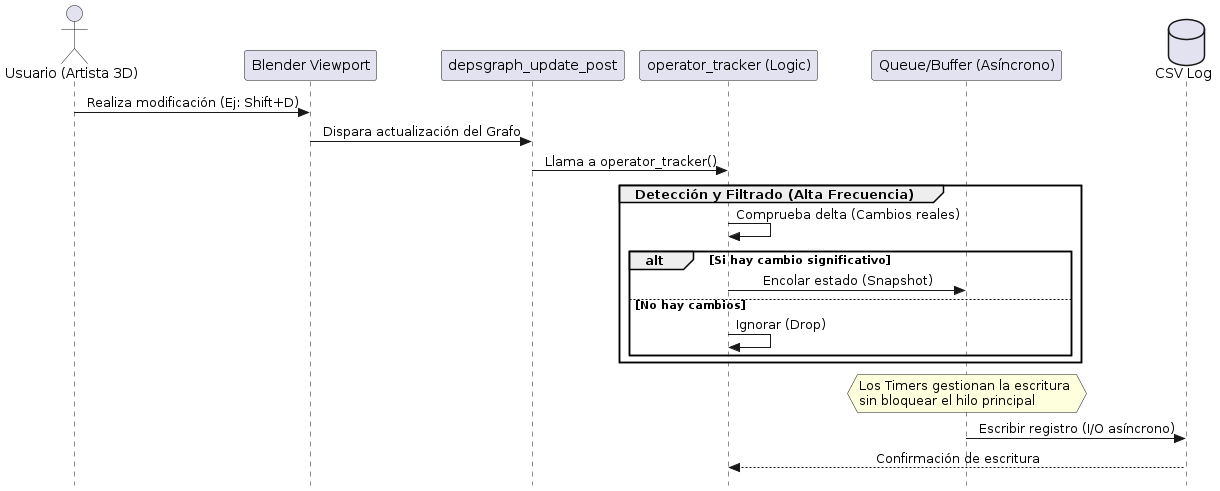
\includegraphics[width=0.85\textwidth]{diagramas/flujo_plan.png}
    \caption{Diagrama de flujo del sistema de captura y análisis planificado.}
    \label{fig:flujo_asincrono}
\end{figure}

\subsection{Lecciones aprendidas}
\label{subsec:a-lecciones-aprendidas}

El proceso de desarrollo ha permitido extraer varias conclusiones técnicas y metodológicas. En primer lugar, la integración con Blender requiere una comprensión detallada del contexto activo, ya que el acceso a la malla, a los operadores y a los datos UV varía según el modo de trabajo. Por este motivo, una parte significativa del esfuerzo se destinó a robustecer la captura antes de ampliar el análisis.

En segundo lugar, el CSV funcionó como un elemento central de la arquitectura. La calidad de las métricas dependía directamente de la estabilidad del formato de datos, por lo que fue necesario normalizar cabeceras, documentar campos y validar valores antes del cálculo.

En tercer lugar, la interfaz necesitó evolucionar junto al sistema. A medida que aumentaba el número de métricas, la presentación inicial resultaba insuficiente. La organización final por pestañas, bloques compactos y tooltips permitió reducir la carga cognitiva del usuario y mejorar la comprensión de los resultados.

Finalmente, la incorporación de optimizaciones como KDTree en métricas geométricas evidenció la importancia de considerar el rendimiento desde fases tempranas. Las comparaciones entre mallas pueden crecer rápidamente en coste computacional, por lo que el uso de estructuras de búsqueda espacial resultó adecuado para mejorar la eficiencia.

\section{Viabilidad del proyecto}
\label{sec:a-viabilidad}

\subsection{Viabilidad técnica}
\label{subsec:a-viabilidad-tecnica}

La viabilidad técnica de la solución queda respaldada por la flexibilidad de Blender como plataforma extensible mediante Python~\cite{pythonlang}. El proyecto se apoya en la API \texttt{bpy}, en operadores personalizados, en manejadores persistentes, en temporizadores y en acceso directo a estructuras de datos de escena.

El primer add-on utiliza módulos estándar de Python y componentes propios de Blender para capturar datos durante la sesión. El uso de \texttt{bmesh} permite acceder a la topología en \textit{Edit Mode}, mientras que \texttt{mathutils} facilita operaciones espaciales sobre matrices, vectores y cajas envolventes.

El segundo add-on resulta técnicamente viable porque el análisis se realiza de forma diferida. Esta decisión evita sobrecargar el proceso de modelado y permite incorporar cálculos más complejos, como:

\begin{itemize}
    \item cálculo de métricas A1--A17 a partir de registros CSV;
    \item validación de datos y control de valores no numéricos;
    \item cálculo de métricas geométricas de malla;
    \item cálculo de métricas UV;
    \item generación de gráficos mediante Matplotlib~\cite{matplotlib};
    \item procesamiento numérico mediante NumPy~\cite{numpy};
    \item optimización de búsquedas espaciales mediante estructuras tipo KDTree cuando procede;
    \item visualización de resultados dentro del entorno de Blender.
\end{itemize}

La principal dificultad técnica procede de la complejidad de la API de Blender y de la necesidad de trabajar con diferentes estados de escena. No obstante, las pruebas iterativas y la refactorización progresiva permitieron alcanzar una solución funcional y extensible.

\subsection{Viabilidad económica}
\label{subsec:a-viabilidad-economica}

Desde el punto de vista económico, el proyecto resulta viable porque se ha desarrollado con tecnologías de código abierto o sin coste directo de licencia. Blender, Python, NumPy, Matplotlib y GitHub en su modalidad básica pueden utilizarse sin costes de adquisición para este contexto académico.

\subsubsection{Costes de software}
\label{subsubsec:a-costes-software}

\begin{itemize}
    \item Blender: 0 €.
    \item Python: 0 €.
    \item GitHub: 0 € en el uso académico básico.
    \item NumPy: 0 €.
    \item Matplotlib: 0 €.
    \item \LaTeX: 0 €.
\end{itemize}

\subsubsection{Costes de hardware}
\label{subsubsec:a-costes-hardware}

Para la ejecución del proyecto se requiere una estación de trabajo capaz de ejecutar Blender de forma fluida. Se toma como referencia un equipo de gama media con un valor estimado de 1200 €. Aplicando una amortización lineal de 48 meses y considerando una dedicación aproximada de cuatro meses al proyecto:

\[
\text{Coste hardware} = \frac{1200}{48} \times 4 = 100\,€
\]

\subsubsection{Coste estimado de desarrollo}
\label{subsubsec:a-costes-desarrollo}

Aunque el proyecto se enmarca en un contexto académico, puede estimarse un coste equivalente de desarrollo tomando como referencia una dedicación de cuatro meses y una remuneración mensual aproximada de 1200 € para un perfil junior:

\[
1200\,€/\text{mes} \times 4\,\text{meses} = 4800\,€
\]

\subsubsection{Coste total estimado}
\label{subsubsec:a-coste-total}

El coste total estimado se obtiene sumando el coste amortizado de hardware y el coste equivalente de desarrollo:

\[
100\,€ + 4800\,€ = 4900\,€
\]

Por tanto, aunque no haya existido un coste directo de licencias, la traslación del proyecto a un entorno profesional tendría un coste aproximado de 4900 €.

\subsection{Viabilidad legal}
\label{subsec:a-viabilidad-legal}

El proyecto se apoya en herramientas y bibliotecas de uso permitido en contextos académicos. Blender se distribuye bajo licencia GNU GPL, Python bajo licencia propia de la Python Software Foundation y las bibliotecas científicas utilizadas cuentan con licencias compatibles con su uso en investigación y desarrollo.

La solución propuesta no modifica el núcleo de Blender, sino que se integra mediante su sistema de add-ons. Desde el punto de vista documental, las referencias externas se incorporan mediante la bibliografía correspondiente y no se incluyen recursos propietarios sin autorización.

\subsection{Viabilidad ética}
\label{subsec:a-viabilidad-etica}

La viabilidad ética del proyecto se fundamenta en la transparencia de la captura y en la minimización de datos personales. El logger registra datos técnicos asociados al proceso de modelado, como transformaciones, cambios topológicos, modos, UV, operadores relevantes y estado de la escena. No registra contenido textual externo, conversaciones, credenciales ni datos personales directos.

Además, el sistema incorpora un mecanismo de consentimiento explícito antes de iniciar la captura. El identificador de usuario se genera de forma seudonimizada, evitando almacenar nombres reales. Aun así, los CSV generados deben tratarse como datos de investigación, ya que pueden reflejar patrones de comportamiento técnico de una persona durante el modelado.

\section{Análisis de riesgos}
\label{sec:a-riesgos}

El desarrollo del proyecto ha estado condicionado por varios riesgos técnicos, funcionales y éticos. La Tabla~\ref{tab:riesgos} recoge los principales riesgos identificados, su impacto y las medidas aplicadas para reducirlos.

\begin{table}[H]
\centering
\scriptsize
\renewcommand{\arraystretch}{1.2}
\begin{tabularx}{\textwidth}{p{3.4cm}p{1.6cm}X}
\toprule
\textbf{Riesgo} & \textbf{Impacto} & \textbf{Medida de mitigación} \\
\midrule
Degradación de rendimiento durante el modelado & Alto & Separación entre captura y análisis, temporizador de muestreo, registro basado en cambios significativos y reducción de operaciones pesadas durante la sesión. \\
Disparidad entre \textit{Object Mode} y \textit{Edit Mode} & Alto & Uso diferenciado de acceso a datos mediante \texttt{obj.data} y \texttt{bmesh.from\_edit\_mesh()} según el modo activo. \\
Crecimiento excesivo del CSV & Medio & Registro diferencial, eliminación de filas duplicadas y escritura solo cuando se detectan cambios relevantes o eventos forzados. \\
Pérdida accidental de datos & Medio & Incrustación del CSV en el archivo \texttt{.blend} y exportación manual a archivo externo. \\
Detección incompleta de operadores & Medio & Normalización de identificadores de operadores, lectura de operadores recientes y uso de banderas específicas para eventos relevantes. \\
Cambios UV no detectados por topología & Medio & Uso de operadores UV conocidos y cálculo de hash global de coordenadas UV. \\
Errores en métricas CSV & Medio & Validación de valores, revisión de funciones de cálculo y pruebas con múltiples CSV y datos reales. \\
Coste elevado en métricas geométricas & Medio & Uso de estructuras de búsqueda espacial como KDTree en cálculos de proximidad y comparación entre mallas. \\
Sobrecarga visual de la interfaz & Bajo & Organización por pestañas, bloques compactos, reducción de textos visibles y uso de tooltips. \\
Riesgos de privacidad & Medio & Consentimiento explícito, seudonimización del identificador y limitación de la captura a datos técnicos. \\
Dependencia de versiones de Blender & Medio & Desarrollo sobre versiones recientes, documentación de dependencias y separación modular para facilitar futuras adaptaciones. \\
\bottomrule
\end{tabularx}
\caption{Matriz de riesgos técnicos, funcionales y éticos del proyecto.}
\label{tab:riesgos}
\end{table}

La aplicación de estas medidas permitió reducir la deuda técnica, mejorar la estabilidad de los add-ons y asegurar una evolución controlada del sistema. En particular, la separación entre logger y análisis fue una decisión clave para mitigar riesgos de rendimiento y facilitar la ampliación posterior de métricas y visualizaciones.

\section{Conclusión del plan de proyecto}
\label{sec:a-conclusion}

El proyecto siguió una planificación iterativa e incremental, aunque la ejecución real presentó ajustes derivados de la complejidad técnica del entorno Blender. La evolución del sistema no fue lineal: algunas tareas de análisis obligaron a revisar la captura, y algunos problemas detectados con datos reales exigieron volver sobre funciones de métricas ya implementadas.

A pesar de estas desviaciones, la planificación permitió mantener una dirección clara. La suite evolucionó desde un logger inicial hasta un sistema formado por dos add-ons complementarios, con captura automática, exportación CSV, análisis estadístico, métricas geométricas, métricas UV, visualizaciones e interfaz organizada por pestañas.

La revisión del historial de commits muestra una progresión coherente: primero se construyó la base del logger, después se normalizó el intercambio de datos, posteriormente se incorporó el análisis, se validaron métricas con datos reales y finalmente se refactorizó el sistema para mejorar rendimiento, mantenibilidad e interfaz. Por tanto, el proyecto puede considerarse viable, trazable y técnicamente coherente con los objetivos planteados.